\documentclass[12pt,english]{article}

\usepackage{natbib}

\usepackage{graphics,graphicx,dcolumn,bm,fleqn,epic,eepic,float}
\usepackage{amssymb,amsmath,multirow,rotate,rotating,color}
\usepackage[utf8]{inputenc}

\usepackage[english]{babel}
\usepackage{caption}
\usepackage{subcaption}
\usepackage{tikz}
\usepackage{hyperref}
\hypersetup{
    colorlinks=true,
    linkcolor=blue,
    filecolor=magenta,      
    urlcolor=cyan,
}
%\usepackage[usenames,dvipsnames,svgnames,table]{xcolor}
\tikzset{fontscale/.style = {font=\relsize{#1}}}
\usetikzlibrary{calc}
\makeatother

\newcommand{\figref}[1]{Fig.~\ref{fig:#1}}
\newcommand{\eqnref}[1]{Eq.~(\ref{eq:#1})}
\newcommand{\ts}{\textsuperscript}

\definecolor{tuered}{RGB}{214,0,74}

\newcommand{\todo}[1]{\textbf{\textcolor{tuered}{ TODO: #1}}}

\newcommand{\vectornorm}[1]{\left|\left|#1\right|\right|}

\renewcommand{\vec}[1]{\mathbf{#1}}
\newcommand{\uvec}[1]{\hat{\vec{#1}}}
\newcommand{\tensor}[1]{\mathbf{#1}}

\definecolor{pyblue}{HTML}{1F77B4}
\definecolor{pyorange}{HTML}{FF7F0C}
\definecolor{pygreen}{HTML}{2CA02C}
\definecolor{pyred}{HTML}{D62728}

\newcommand{\JH}[1]{\textcolor{blue}{JH: #1}}
\begin{document}

% The referee PDF has been generated from r239 -- 'make referee' command.

\section*{Reply to Referee A}
We thank the Referee for his/her report on our manuscript. 
We are glad to read that he/she finds it of potential interest and in principle 
suitable of publication, if a thorough revision is performed. 
This is what we did in the new version, where we tried to clarify the obscure points, following all the Referee's remarks.
Hereafter we provided answers to the various questions/comments raised. All changes in the revised 
version are reported in red colour.

\begin{itemize}

\item[ \textbf{\underline{Comment 1.}}]
{ 
I am unable to follow most of the arguments made with respect to the disjoining pressure. 
For me, one needs to integrate the disjoining pressure to arrive at an effective interface potential, and 
I do not really know how to go from the effective interface potential to the surface tension. 
The equation (3) therefore merits much more discussion.
}

\item[ \textbf{{Answer}}]
{
We did not give, in fact, any particular argument with respect to the disjoining pressure, since 
we assumed that it is a very well established concept employed in any theoretical and computational study of thin liquid film hydrodynamic in the lubrication approximation framework.
We acknowledge, though, that our assumption was probably erroneous and we give some more explanation. 
First of all, there is no need (and no way) to go from the disjoining pressure (or the interface potential) to the surface tension, since the two quantities carry complementary physical information. 
Let us, first, make a step back and underline a fundamental difference between the physics of {\it one free interface} and that of a {\it film}:
the latter is a layer of liquid confined between {\it two} interfaces. When the two interfaces are brought close enough to each other (the layer is thin), they interact.
The disjoining pressure stems from the interaction. Thermodynamically, it represents minus the derivative of the free energy difference, per unit surface, between 
the film and the bulk of the same liquid, or, equivalently, the pressure difference inside and outside the film 
\cite{Deryaguin1936,DeryaguinChuraev1978}.
In the case of wetting, there can be three types of interfaces: liquid/air, liquid/solid (the substrate) and, 
if the substrate is only partially wetted, solid/air, thus giving rise to three-phase contact lines. 
The usually called {\it surface tension} is the energy cost of forming a liquid/air interface of unit area and its only knowledge is, therefore, not enough in our case. 
The Young's condition (Young, 1805, de Gennes, 1985) connects the surface tension with the analogous energies per unit
area associated with the solid/liquid ($\gamma_{\text{sl}}$) and solid/gas ($\gamma_{\text{sg}}$) interface as
\begin{equation}
\cos \theta = \frac{\gamma_{\text{sg}}-\gamma_{\text{sl}}}{\gamma},
\end{equation}
where $\theta$ is the contact angle.
So, there is no need (and no way) to go from the disjoining pressure (or the interface potential) to the surface tension, since the two quantities carry complementary physical information,
and both are required to determine the dynamics of dewetting.
Of course, on the other hand, the disjoining pressure depends also on the surface tension, which appears, in fact, in its expression (3). 
We think, though, that part of the confusion might be due to the fact that we do not define the symbol of the surface tension at its first occurrence, but only later. 
We have now fixed this and we apologize for it.
}

\item[ \textbf{\underline{Comment 2.}}] 
{
The same holds for the time scale. 
The viscous time scale is well defined, but necessitates a length scale in addition to the 
capillary velocity. It is unclear why the authors choose the length scale that they use in the paper.
Subsequently, they replace the surface tension by a complicated partial derivative of the 
disjoining pressure; here the same remark as above holds.
}

\item[ \textbf{{Answer}}]
{
We apologize if we have not been thorough in the discussion of the relevant scales, which indeed deserves some clarification. 
Thin film hydrodynamics is an intrinsically multiscale phenomenon, whereby there are at least two characteristic length scales: the mean film thickness (let us call it $h_0$)
and an horizontal length scale $\ell$ (which in our case can be, for example, the pattern wavelength, $\lambda$), where, typically $h_0 \ll \ell$. We chose to use the mean 
film thickness as a scale, because it is the only relevant length that is common to all the simulations.
In the same spirit, we chose as a reference time, $t_0(\theta)$, which is not exactly the capillary time (though being related to it). 
$t_0$, as we explain in the text, is, in fact, the characteristic time of growth of the most unstable mode in the spinodal dewetting on a homogeneous
substrate of contact angle $\theta$. In spite of the substrate being patterned in our case, it is possible to define an effective $t_0$ in terms 
of the highest contact angle on the pattern, which is what determines the fastest instability, i.e. $t_0(\Theta)$, where 
$\Theta=\mbox{max}_{\mathbf{x}}\{\theta(\mathbf{x})\}= \theta_0 + \delta \theta$. We deem the so defined characteristic time as an appropriate scale,
since it does not depend on the pattern wavelength and speed. Actually, one can see that it captures well the time scales of the dewetting process
from figure 2, where it is shown that the rupture times are of the order of fraction to units of $t_0$.
We recognize, on the other hand, that, in this spirit it is unclear the reason of the choice of $v_0 = \lambda/t_0$ as a reference velocity.
A more natural candidate would be, indeed, $v_0=h_0/t_0$. We have therefore decided to use the latter in the revised version of the manuscript.
We have also rephrased the corresponding paragraph in the {\it Method} section as follows: \\

\textcolor{red}{}

}

\item[ \textbf{\underline{Comment 3.}}]
{ 
Incidentally, for a 'normal' fluid such as water, the capillary velocity is $\sim 70\mbox{m}/\mbox{s}$, 
so that very, very rapidly the fluid inertia becomes important. 
This is indeed what one usually observes for the formation or coalescence of drops, so that at the very least this should be discussed and the Reynolds number calculated.
}

\item[ \textbf{{Answer}}]
{
Such a high value corresponds to the ratio of (surface tension)/(dynamic viscosity) for water, i.e. $v = \gamma/\eta \approx 70 \mbox{m}/\mbox{s}$.
This expression, though, is only representative of the capillary velocity, again, for {\it free surface flows}, as, e.g., in the coalescence of 
two droplets in the bulk of another fluid. In the case of thin liquid films, the capillary velocity is still proportional to the ratio 
$\gamma/\eta$, but by a factor $\varepsilon^3$, where $\varepsilon = h_0/L$ is the film thichkness parameter, which is typically $\varepsilon \ll 1$.
For the dewetting of a millimetric film of micrometric thickness reatracting into a single droplet, experiments have measured that 
the typical velocity is $\sim 1 \mbox{mm}/\mbox{s}$, which gives a Reynolds number $Re \approx 10^{-3}$ \cite{Edwards}.
}

\item[ \textbf{\underline{Comment 4.}}]
{ 
In addition, there is a lot of old literature that relates the dewetting to the disjoining pressure, and shows that the nucleation of a hole in a wetting film is much more difficult than the nucleation of such a wetting film; there are experiments on this by Rutledge and Taborek, theory by Schick and Taborek and Bausch, Blossey and Indekeu.
}

\item[ \textbf{{Answer}}]
{
We thank the referee for bringing this to our attention.
However, we have hard time understanding what he/she means with ``\textit{... and shows that the nucleation of a hole in a wetting film is much more difficult than the nucleation of such a wetting film}''
}

\item[ \textbf{\underline{Comment 8.}}]
{ 
The explanations also lack a discussion on time, length, and energy scales. 
}

\item[ \textbf{{Answer}}]
{
We find this comment odd as we provide suitable time and length scales, derived from the disjoining pressure.
A natural energy scale emerges as the spreading parameter $\mathcal{S}$ which can be derived from the disjoining pressure as well. 
We are very sorry if the referee dislikes the model of the disjoining pressure, but various publications can be found using this model, see answer to Comment 2.
}

\item[ \textbf{\underline{Comment 9.}}]
{ 
I have no clue what the values mean ``the numerical values, in LB units, are set to $\gamma= 0.01$ and  $\mu = 1/6$''. 
}

\item[ \textbf{{Answer}}]
{
We are sorry to hear that these numbers have led to confusion.
For completeness of the manuscript, we provide the parameters (and the code, see arXiv) we used to generate data.
The referee is right to question these numbers, and we agree that their values seem arbitrary.
Using the lattice Boltzmann method, it can be shown that the choice of $\mu = 1/6$ is the most stable for a single relaxation time collision operator~\cite{kruger2017lattice}.

To make sense of them, we scale them with characteristic quantities of a dewetting thin film, therefore $q_0$ and $t_0$.
}

\item[ \textbf{\underline{Comment 10.}}]
{ 
What is the disjoining pressure due to? 
Van der Waals forces? 
How thick is the precursor film, and why should the disjoining pressure be zero there?
Is there any comparison with experiments possible/feasible?
}

\item[ \textbf{{Answer}}]
{
The disjoining pressure allows us to have an effective three phase contact line with the correct wetting behavior and without diverging pressure.
We agree that this a purely numerical problem that does not appear in experiments, although it is possible to relate the disjoing pressure to the Hamaker constant,
\begin{equation*}
    \mathcal{A} = 6\pi h^3\kappa(\theta),
\end{equation*}
using 
\begin{equation*}
    \kappa(\theta) = \frac{2\gamma}{h_{\ast}}(1-\cos(\theta(\mathbf{x},t))),
\end{equation*}
which is non powerlaw part of the disjoining pressure.

Advancing three phase contact lines are a topic by its own, and we would point the referee towards relevant literature, as this discussion would be beyond the scope of the problem at hand.

The referee is correct in assuming it includes Van der Waals forces.
This is another very interesting comment, as far as the authors can tell there is no common sense on the existence of the precursor layer.
There are experimental studied that claim its existence, but with a thickness of only a few nanometers.
In our model it mainly ensures that the pressure near the three phase contact line is well behaved.
There is actually a lot of comparison with experiments see refs.~\cite{becker2003complex, fetzer2007thermal, doi:10.1073/pnas.1820487116} or e.g. the review from Bonn et al.~\cite{RevModPhys.81.739}.
We would further refer to the answer of Comment 2.
}

\end{itemize}

\section*{Reply to Referee B}

We thank the Referee for his/her thorough reading of our manuscript and detailed report.
We are happy to read that the referee acknowledges the amount of work we did and thinks it could be fitting for PRL after revision.
In what follows we provide detailed answers to all Referee's questions and we discuss all the changes made to the manuscript
(which are written in the text in red colour).

\begin{itemize}


\item[ \textbf{\underline{Comment 1.}}]
{
The model disjoining pressure, Eq. 3 with a tail decaying as the inverse squared power seems odd. 
I am more familiar with the expected van der Waals tail with a decay as the inverse cube power. 
Is there any reason for this choice?

\item[ \textbf{Answer}]
{
We thank the referee for pointing this out.
It is true that there are variations concerning the powerlaw model of the disjoining pressure.
A common one to which the referee refers to is $(n,m) = (9,3)$, the choice we made for the manuscript is $(n,m) = (3,2)$.
Both exponent pairs can be found in the literature with even more variety~\cite{moulton_lega_2013,SCHWARTZ1998173,doi:10.1063/1.4828721,brasjen2013dewetting}.
The pair $(9,3)$ is the one that can be motivated from functional derivatives of a Lenard-Jones potential, understandably this could more appealing to use.
We have used both exponent pairs in previous works, see e.g.~\cite{PhysRevE.104.034801}.
In this manuscript we used $(3,2)$ to keep $t_0$ reasonably small and thus the overall computational cost manageable.
Using the pair $(9,3)$ does not alter the results, it effectively shifts the value of $t_0$ by $\approx 10$.
}

\item[ \textbf{\underline{Comment 3.}}]
The second major concern refers to the choice of slip length. 
The authors study a fluid-substrate model that has a thin film equilibrium thickness of 0.07 length units, but the slip length is one unit, hence about 10 times larger than the equilibrium film thickness. 
This seems unexpected, in view of the small contact angle chosen for the system. 
Could the authors justify this choice?
}

\item[ \textbf{Answer}]
{
\begin{figure}
    \centering
    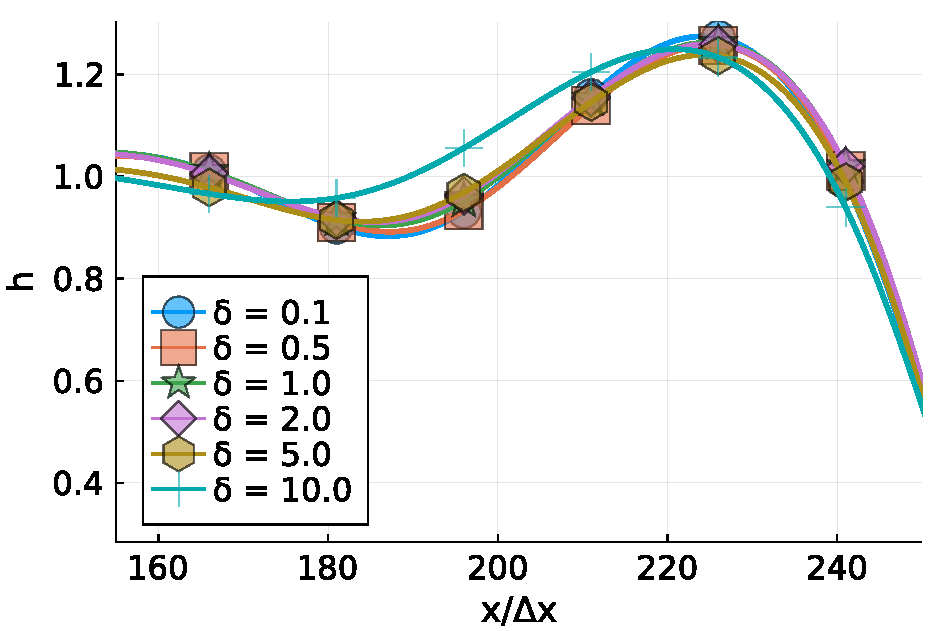
\includegraphics [width=0.6\textwidth]{slip_measure.pdf}
    \caption{Dewetting rim profiles for various slip parameters $\delta$.}
    \label{fig:slip}
\end{figure}

We thank the referee for bringing this up and are happy to talk about this issue.
Slip and disjoining pressure are an essential part of our model, and many other thin film solvers.
Here they allow us to have moving contact lines with imposed wettability features.

We agree that the value may seem large at first glance.
As Peschka et al. have shown, the creation of satellite droplets during rivulet breakup, similar to what we observe, is a no-slip feature~\cite{doi:10.1073/pnas.1820487116}.
We observe the creation of satellite droplets in the initial dewetting.
Increasing the slip length makes those droplets disappear.

Another point to mention here is the slip dependency of the dewetting rim.
Small to vanishing slip induce a dimple behind the front, while for large slip values this dimple vanishes~\cite{fetzer2007quantifying, munch2005contact}.
We checked this behaviour in Fig.~\ref{fig:slip} and found only a small dependency for slip lengths $\delta < 10$.

Spots with thickness $h \leq h_{\ast}$ are considered dry spots, therefore the term equilibrium thickness maybe exaturated.
}

\item[ \textbf{\underline{Comment 4.}}]
{
The relevance of the manuscript relies on the significance of the substrate's switchable properties. 
Particularly, it is assumed that the wetting properties can be modulated on space but also on time. 
The authors have mentioned in the introduction that this can be potentially done. 
However, it would be desirable that the authors relate their model of switchable substrate with some specific experimental realization, where the actual length and time scales are mentioned.
}

\item[ \textbf{{Answer}}]
{
\begin{figure}
    \centering
    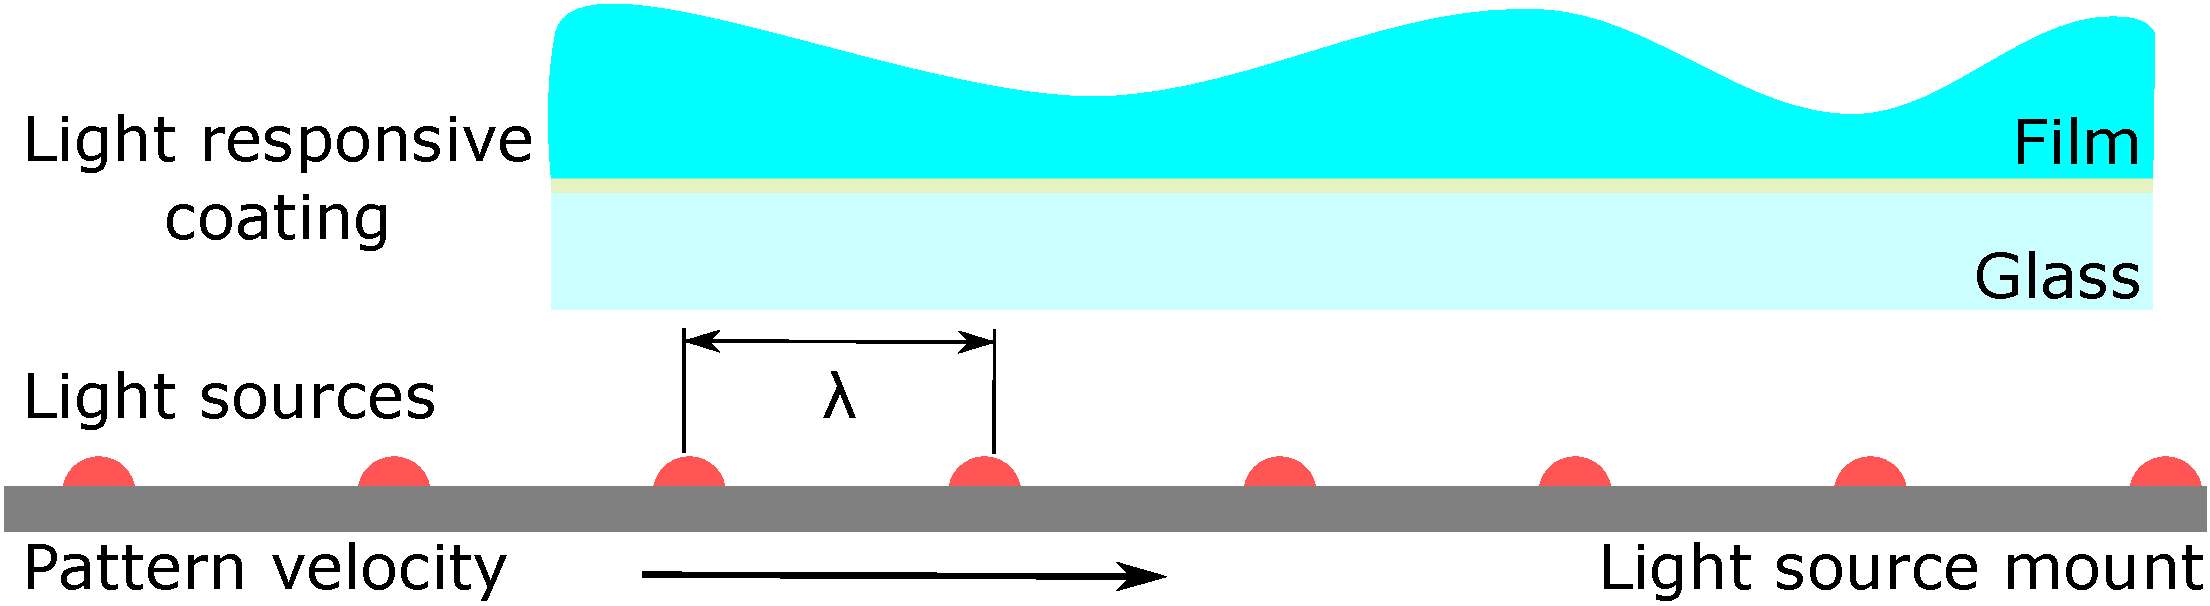
\includegraphics[width=\textwidth]{simple_exp.pdf}
    \caption{Schematic realization of the experiment described in the manuscript.}
    \label{fig:experiment_illustration}
\end{figure}
We thank the referee for bringing this up.
First, we like to note that experiments are not our field of expertise and therefore our envisioned realization could be flawed.

The idea we have would be to prepare a thin film ($h_0 \approx 4nm$ PS) on a light responsive substrate.
Dimensions of the substrate should at least be $2$ microns in $x$ and $y$, but larger is fine.
Arrange several light sources (diodes) in a lattice with a distance of $\lambda \approx 1\mu m$ between them, as displayed in Fig.~\ref{fig:experiment_illustration}.
It would be perfect if the structure on which the light sources are mounted can be moved in a periodic manner, e.g. wrapped around rolls.
On the other hand if the array of diodes is large enough, say $100\lambda$ it should be sufficient to move them continuously in one direction. 

In Eq.~(5) we introduce two scales, $t_0$ and $v_0$.
From experiments of dewetting thin films we know that $t_0$ correlates with the rupture time~\cite{becker2003complex, fetzer2007thermal}.
Considering the same experimental parameters as above, 
\begin{align*}
    t_0 &\approx 1800s,\qquad~~~\qquad \frac{2\pi}{q_0}\approx 400nm, \\
    \quad v_0 &= \frac{\lambda}{t_0} \approx \frac{1}{900}\frac{\mu m}{s},\quad \quad v_0^{\ast} = \frac{2\pi}{q_0 t_0} \approx \frac{4}{9}\frac{nm}{s},
\end{align*}
where we take into account that the rupture time is overestimated by about a factor of two.
The experiment therefore reduces to the movement of the diodes with a velocity between $[10^{-7}/900, 10^{-5}/900] m/s$. 
}

\item[ \textbf{\underline{Comment 5.}}]
{
An important parameter in the problem is the wave-vector $q_0$, which sets the correlation length in the problem. 
The authors should state what the actual value is relative to either the average film height, or the wave-length of modulations. 
Is there any reason to give the wave-length of modulations in units of the system size, i.e., are the results subject to finite size effects? Otherwise it appears more meaningful to describe the modulations in units of $q_0$ or the equilibrium film thickness.
}

\item[ \textbf{{Answer}}]
{
We thank the referee for this comment.
It is true that we use $q_0$ but never display its actual value.
Inserting numbers, we have 
\begin{equation*}
    q_0 \approx 0.13, \quad \lambda_0 = \frac{2\pi}{q_0} \approx 48.5 \approx \frac{L}{10},  
\end{equation*}
therefore $\lambda_0$ is usually smaller than $\lambda$.

No, these simulations do not suffer from finite size effects.
The honest reason for using multiples of the system size is the ease of the numerical realization.
Having periodic boundary conditions, a non-multiple wavelength of the system size would induce a discontinuity.
Given the complexity of the problem, we would like to have as much control of the pattern as possible.

The arbitrary choice we made had however helped us to understand where the boundary between rivulet and droplets appear.
In Eq.~(11) we use
\begin{equation*}
    \Gamma = \frac{v_{\theta}}{U_{\theta}} = \frac{\chi v_0}{U_{\theta}},
\end{equation*}
where rivulets appear for $\chi > 1$.
Substituting the wavelength dependence of $v_0$ with $q_0$,
\begin{equation*}
    v_0^{\ast} = \frac{\lambda_0}{t_0}, 
\end{equation*}
computing $\Gamma$ in terms of $v_0^{\ast}$ yields
\begin{equation*}
    \Gamma = \frac{v_0^{\ast}}{U_{\theta}} = \frac{6\pi h_0^3 q_0^3}{\Theta^3},
\end{equation*}
relating both with each other yields
\begin{equation*}
    \frac{\chi 3\lambda h_0^3 q_0^4}{\Theta^3} = \frac{6\pi h_0^3 q_0^3}{\Theta^3},
\end{equation*}
with most of the terms canceling one gets
\begin{equation*}
    \lambda = \frac{2\pi}{q_0\chi}, 
\end{equation*}
which in fact state that if the wavelength $\chi^{-1}2\pi/q_0 < \lambda$ rivulets should form. 
}

\item[ \textbf{\underline{Comment 6.}}]
{
The thin film equation relies on a local approximation for the interface potential and disjoining pressure. 
Notice that to first order in non-local effects, the surface tension entering the thin film equation adopts a film thickness dependence which could potentially affect the dynamics. 
Particularly, as far as the parallel correlation length $q_0$ is referred, the non-local effects provide an upper bound equal to the inverse bulk correlation length. 
This could be a significant effect in polymer thin films (c.f. Benet et al. jpc-c 118, 22079, 2014 and the related discussion on dynamical effects Pahlavan et al., jfm, 845, 642, 2018).
}

\item[ \textbf{{Answer}}]
{
That is indeed a very interesting point.
In fact, we know the second reference very well from our own work~\cite{PhysRevE.104.034801}.
It is an appealing model, and we look forward to discussing it in further details in future publications.
We therefore added the following to the conclusion 
\\
\textcolor{red}{Never gonna give you up\\
Never gonna let you down\\
Never gonna run around and desert you\\
Never gonna make you cry\\
Never gonna say goodbye\\
Never gonna tell a lie and hurt you}
}

\end{itemize}

\section*{Reply to Referee C}
We thank the Referee for his/her report on our manuscript.
It is a pleasure to read that he/she acknowledges the credibility of the work and finds our writing appealing.
We are happy to see the he/she likes the interpretation of our results in terms of scaling arguments.
In what follows we provide detailed answers to all Referee's questions and we discuss all the changes made to the manuscript
(which are written in the text in red colour).

\begin{itemize}

\item[ \textbf{\underline{Comment 1.}}]
{ 
The topic may be potentially relevant for microfluidic and related applications journals, e.g., Physical Review E or Physical Review Fluids.
}

\item[ \textbf{{Answer}}]
{ 
We think this comment is judgmental, and it relates neither to the quality of the manuscript nor to the findings of the manuscript.
It is a statement about personal preference and belittles work which was published in Physical Review Letters on dewetting~\cite{fetzer2007thermal}, microfludic~\cite{PhysRevLett.110.048303} and thin film morphologies~\cite{PhysRevLett.84.931}.
Given the novelty of the dewetting interaction with the modelled ``switchable substrate'' we truly think that our findings fit the scope of Physical Review Letters.
}

\item[ \textbf{\underline{Comment 2.}}]
{ 
However, I feel that the results presented lack a sufficient breadth and impact so as to warrant publication in Physical Review Letters - provided that one has a suitable substrate, I do not see how would the transport of a fluid by way of transient rivulets surpass the transport by way of droplets in practice - and thus I cannot recommend the manuscript for publication.
}

\item[ \textbf{{Answer}}]
{ 
We understand that the referee expresses his/her point of view and acknowledge it.
However, we find it odd that he/she would disregard a result because there is no immediate use case that comes to his/her mind.
Scientific work is creative work, solving unsolved problems to deepen our understanding of the world.
To the best of our knowledge, this manuscript describes an effect that has not been observed so far and is accompanied by theoretical justification.

The referee raises the point that transport using rivulets can not surpass transport by droplets.
We have to disagree with this comment.
Transporting droplets on a patterned substrate is a difficult task, with many hideous effects such as contact line pinning or pearling/coalescence~\cite{PhysRevLett.119.204501}.
The contact line of a rivulet on the other hand is simpler can can only if at all move along the flow direction.
Therefore, the authors think that there can be cases for which transport via rivulet could be favorable.

Apart from the transport problem, controlling the morphology of small volumes of fluids is a highly desired application.
From a purely theoretical point of view it is an interesting question of how to overcome the surface energy minimization due to droplet fragmentation. 
Printing integrated circuits only by the means of a dewetting thin film, without having to use lithography, sounds for example very appealing.
What we want to say is that a singular opinion may not cover the whole space of possible applications, be it in a scientific set up or an industrial.
}

\item[ \textbf{\underline{Comment 3.}}]
{ 
For example, I imagine that the rivulets will not form if $\delta\theta$ were too small, or too small relative to $\theta_0$. 
The authors focused on the importance of the speed of the pattern and on its wavelength but they left most other parameters fixed to a single value, the reasons for their choice being unclear.
}

\item[ \textbf{{Answer}}]
{ 
The observation of the referee is correct.
Indeed, the difference in contact angle amounts to a net force on the liquid.
This force can be large enough to actuate droplets~\cite{doi:10.1021/acs.langmuir.5b02335}.

The thin film equation is valid only in the regime where $\theta \ll \pi/2$.
Choosing $\theta_0 = 20^{\circ}$ and a $\Delta\theta$ of the same magnitude therefore ensures that we are well within the predictability of our model.
Therefore we find that our value of $\theta_0$ is a good compromise to satisfying the constraints.

Most of our results are given in terms of $t_0$ and $q_0$.
Both contain parameters we choose to set up our numerical experiments. 
We supply an equation to calculate them and have no evidence to believe that our theoretical assumptions are incorrect.
Could the referee please elaborate why he/she thinks we overlook something?

\textcolor{pyorange}{Stefan}: I would put the results we have from the x-only velocity run here.
They kind a answer what happens if $\Delta\theta$ becomes larger (rivulets life for a very short amount of time only).
}

\item[ \textbf{\underline{Comment 4.}}]
{ 
Also unclear is how does the substrate patterning scale $2\pi/q_\theta$ compare with the scale of homogeneous dewetting $2\pi/q_0$.
I tried hard to understand whether the different cases of $\lambda$ discussed in the paper agree with $2\pi/q_0$ but I was unable to do so. 
}

\item[ \textbf{{Answer}}]
{ 
We are sorry for creating confusion with the choice of our variables.
Let us call $\lambda_0 = 2\pi/q_0$ and rephrase Eq.~(11) in terms of $\lambda_0$ using $v_0^{\ast}$,
\begin{equation*}
    v_0^{\ast} = \frac{\lambda_0}{t_0}, 
\end{equation*}
computing $\Gamma$ in terms of $v_0^{\ast}$ yields
\begin{equation*}
    \Gamma = \frac{v_0^{\ast}}{U_{\theta}} = \frac{6\pi h_0^3 q_0^3}{\Theta^3}.
\end{equation*}
Setting this result equal with Eq.~(11) in the manuscript we have
\begin{equation*}
    \frac{\chi 3\lambda h_0^3 q_0^4}{\Theta^3} = \frac{6\pi h_0^3 q_0^3}{\Theta^3},
\end{equation*}
with most of the terms canceling
\begin{equation*}
    \lambda = \frac{2\pi}{q_0\chi}, 
\end{equation*}
which in fact state that if the wavelength $\chi^{-1}2\pi/q_0 < \lambda$ rivulets should form. 
}

\item[ \textbf{\underline{Comment 5.}}]
{ 
How would the film behave if the dynamics of the film were controlled primarily by spinodal dewetting and not by the contact-angle pattern?
}

\item[ \textbf{{Answer}}]
{ 
We thank the referee for raising this question.
The straightforward answer is we can reproduce the structure factor of a spinodally dewetting thin film which is given by
\begin{equation*}
    S(q,t) = S_0 e^{2\omega(q)t},
\end{equation*}
where is $S_0$ is a constant factor and 
\begin{equation*}
    \omega(q) = \frac{1}{t_0}\left[2\left(\frac{q}{q_0}\right)^2 - \left(\frac{q}{q_0}\right)^4\right],
\end{equation*}
}
which can be found in ref.~\cite{PhysRevE.104.034801}, Fig~1.
After the generation of droplets, we observe a coarsening scaling according to a powerlaw.

\item[ \textbf{\underline{Comment 6.}}]
{ 
At the same time, if the two characteristic lengthscales (= that of the spinodal dewetting and that of the patterned substrate) are suitably synchronized, perhaps rivulets can be rendered permanent rather than transient?
}

\item[ \textbf{{Answer}}]
{ 
This is an interesting comment.
To our understanding, this is not the case as shown in Fig.~5 of the manuscript.
We observe a saturation like effect for high pattern velocity.
Independent of the velocities, the rivulet admits a varicose instability, which within our study was not possible to overcome.
We hypothesize that another substrate pattern could ensure indefinite rivulet stability.
However as we do not have an intuition, testing N-patterns would be beyond the scope of this work.

For further details on the scale synchronization, we would point towards the answer to Comment 4.
}

\item[ \textbf{\underline{Comment 7.}}]
{ 
Or is the dewetting, once initiated, immanently irreversible even for a time-dependent contact-angle pattern like the one studied in LM17723?
}

\item[ \textbf{{Answer}}]
{ 
That is a very interesting question.
It could be possible, assuming
\begin{equation*}
    \theta(\mathbf{x},t)|_{t > 5t_0} = 0.    
\end{equation*}
We don't think that it is reversible for a non fully wetting substrate.

}

\item[ \textbf{\underline{Comment 8.}}]
{ 
For example, the linear and the square scaling laws in Fig. 2 each cover a small range (much less than a tenfold variation) and so it is hard to see whether they really apply.
}

\item[ \textbf{{Answer}}]
{ 
We agree with the referee and are sorry for the lack of data.
On the upper end we are limited by the total domain of our simulation, otherwise we lose periodicity.
We would like to keep periodicity otherwise sharp wetting gradients appear, see ref.~\cite{PhysRevE.104.034801} for their influence.
On the lower end, we need sufficiently many lattice points to resolve $\sin(x)$.
This is why we comprimise and display two theoretically valid powerlaws in less than tenfold variation.
}

\item[ \textbf{\underline{Comment 9.}}]
{ 
The same goes for the rivulet lifetime in Fig. 5 where the trend is OK but most likely a scaling law different from $\log(v_{\theta})$ would do as well in the range of $\tau_{riv}$ covered by the numerical data.
}

\item[ \textbf{{Answer}}]
{ 
We agree that another powerlaw could fit the data as well.
On the lower end we are bound to the appearance of rivulets, thus $v_{\theta} > 1$ or $v_0^{\ast} < \lambda$.
While in the upper end we observe a saturation explained in the answer to Comment 6.

Theoretically, this seems to be the easiest explanation to our data.
In Comment 3 the referee correctly observes that we have a well-defined protocol where we only change wavelength and pattern velocity.
Any powerlaw that does not correlate with the pattern wavelength would therefore not capture our observations.
}


\end{itemize}

\bibliographystyle{abbrv}
\bibliography{Ref}

\end{document}
